\chapter{\textbf{Marco teórico}}

\thispagestyle{empty}

En este capítulo se presentan los aspectos teóricos que sustentan y respaldan el desarrollo del proyecto de pasantía. A continuación se describen los conceptos que permiten explicar el problema planteado.

\section{Auditoría}

Es una revisión sistemática para determinar si la calidad de las actividades cumplen con los acuerdos planificados y si estos están implementados efectivamente y son adecuados para alcanzar sus objetivos. Ofrecen una oportunidad de mejora al sistema y pueden ser llevadas a cabo para cumplir con normas regulatorias. Las auditorías se pueden aplicar a sistemas, procesos, programas o servicios y pueden ser internas (realizadas por la misma empresa) o externas (realizadas por proveedores) \cite{weinstein1997total}.

\section{Acciones auditables}

Se considera una acción auditable todo flujo del sistema que cree, edite o borre alguna información sensible para el mundo de negocio. Son registradas incluyendo información sobre quién realizó la acción, qué acción se intentó realizar y cuándo ocurrió la acción.

\section{Microservicio}

Es un tipo de arquitectura que consiste en desarrollar una aplicación como un conjunto de pequeños servicios. Dichos servicios son procesos autónomos, cohesivos e independientes que suelen interactuar con otros componentes a través de mensajes \cite{Microservices1}. Se enfocan en resolver un único problema y funcionan de manera aislada; si se presentan una falla no se propaga y puede ser atendido más rápidamente \cite{Microservices2}. \\

Estos servicios se manejan de manera descentralizada y hacen uso de un despliegue completamente automatizado. Cada uno de ellos pueden ser escritos en diferentes lenguajes y tecnologías para almacenar información y aún así, interactuar y compartir información \cite{Microservices2}.

\section{Integración Contínua}

Es una práctica de desarrollo de \textit{software} en la que los miembros del equipo combinan su trabajo de forma periódica, usualmente cada día. Cada integración está verificada por una herramienta automatizada que empaquete y pruebe el código para detectar errores lo más rápido posible \cite{Integracion_Continua}, de esta manera se puede mejorar la calidad del \textit{software} y reducir el tiempo en validar y publicar actualizaciones.

\section{Pruebas automatizadas}

Las pruebas tienen como objetivo ejercitar el código para detectar errores y verificar que el \textit{software} satisface los requerimientos especificados para asegurar su calidad. Estas son realizadas desde el punto de vista del usuario y las funcionalidades son probadas ingresando información y examinando la salida \cite{Pruebas_Automatizadas}. \\

Esta labor puede ser larga y repetitiva, por lo que es conveniente contar con herramientas que provean métodos que faciliten el proceso de escribir y  ejecutar casos de prueba y así, reducir significativamente el esfuerzo y tiempo invertido por los desarrolladores \cite{Pruebas_Automatizadas}. A este conjunto de casos de pruebas se le conoce como prueba automatizada.

\section{Patrón Modelo-Vista-Controlador}

Este patrón de diseño asigna objetos en una aplicación a uno de tres roles: modelo, vista o controlador y define cómo se comunican entre ellos. La colección de objetos de cada tipo puede ser referido como una “capa” \cite{MVC}.

\begin{itemize}
    \item Modelo: controla el comportamiento y la data de la aplicación, responde las solicitudes de información (usualmente desde la vista) y las instrucciones de cambio de estado (usualmente desde el controlador).
    \item Vista: maneja la presentación de la información.
    \item Controlador: interpreta las entradas del usuario y le informa al modelo y/o vista para cambiar lo que sea apropiado \cite{MVC1}.
\end{itemize}

\begin{figure}[h]
\centering
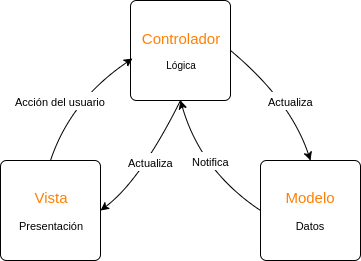
\includegraphics[width=0.5\textwidth]{MVC.png}
\caption{Diagrama del patrón MVC (creación propia).}
\label{fig:figura3.1}
\end{figure}

Es importante notar que la vista y el controlador dependen del modelo, sin embargo el modelo es independiente. Esta separación permite probar el modelo aparte de la presentación visual.

\section{Patrón Modelo-Vista-Plantilla}

Es una adaptación del patrón MVC, en el cual la “vista” define cuál dato es presentado y su comportamiento, no como se muestra. El dato es obtenido a través de la función de \textit{callback} para pedir una URL en particular. Por otro lado, la “vista” delega a la “plantilla”  la presentación de la información.\\

En el caso de Django, el “controlador” es el \textit{framework} en sí: “la maquinaria que envía una petición a la vista apropiada, de acuerdo a la configuración de URL de Django” \cite{MVT}.

\begin{figure}[h]
\centering
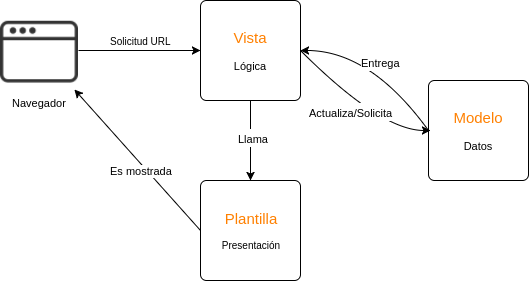
\includegraphics[width=0.7\textwidth]{MVT.png}
\caption{Diagrama del patrón MVT (creación propia).}
\label{fig:figura3.2}
\end{figure}

\section{Señales}

Permiten a las aplicaciones ser notificadas cuando ocurra una acción en algún otro lugar, es decir, las señales permiten a ciertos emisores notificar a un conjunto de receptores que alguna acción está siendo ejecutada \cite{Signals}. En términos de \textit{software}, son el análogo a interrupciones de \textit{hardware} \cite{Senales}.

\section{Mixins}

Es un estilo de programación en el cual las unidades de funcionalidad son creadas en una clase y se incorporan en otras \cite{Mixins}. Pueden entenderse como “un subclase abstracta que puede ser usada para especializar el comportamiento de una variedad de padres” \cite{Mixins2}. \\

Usualmente, los \textit{Mixins}, definen nuevos métodos que realizan alguna acción y luego llaman a los métodos del padre correspondiente; pueden utilizarse en varias clases de la jerarquía y sin importar en qué clases sean usadas. \\

Hay varias razones para usar \textit{Mixins}: extienden las clases existentes sin tener que editar, mantener o combinar el código fuente; mantienen el proyecto en componentes separados; facilitan la creación de nuevas clases con funcionalidades pre-fabricadas y que se puede combinar según sea la necesidad \cite{Mixins}.

\section{Serializadores}

La \textit{Serialization} es un proceso que consiste en convertir un objeto en
un formato que sea fácilmente transmitido a través de la red o que pueda
alojarse en un lugar de almacenamiento consistente (i.e base de datos). Los
\textit{serializers} pueden ser utilizados, simplemente, para que un objeto sea
legible por humanos.
